\section{Aufbau}
\label{sec:Aufbau}

Die schematische Darstellung des Versuchsaufbau ist in Abbildung \ref{fig:aufbau} zu sehen. An der Probe, ein Kupferblock mit einer Masse von \SI{342}{\gram},  ist eine Heizwicklung sowie ein Pt-100 Messwiederstand zur Bestimmung der Temperatur angebracht.
Mit der Funktion
\begin{equation}
	T = 0,00134 R^2 + 2,296 R -243,02
	\label{eq:pt100}
\end{equation}
lässt sich aus dessen Widerstand die Temperatur in °C bestimmen.
 Sie befindet sich in einem Rezipienten, welcher ebenfalls geheizt werden, sowie evakuiert und mit Helium gefüllt werden kann. Der Rezipient befindet sich in einem Dewar-Gefäß, das zu Beginn des Versuches mit flüssigen Stickstoff befüllt wird. Für den Messvorgang sind die Messwiderstände mit einem Ohmmetern verbunden.
Zur Bestimmung der zugeführten Wärmemenge sind die Heizwicklungen mit integrierten Volt- bzw. Ampermeter angeschlossen.

\begin{figure}
  \centering
  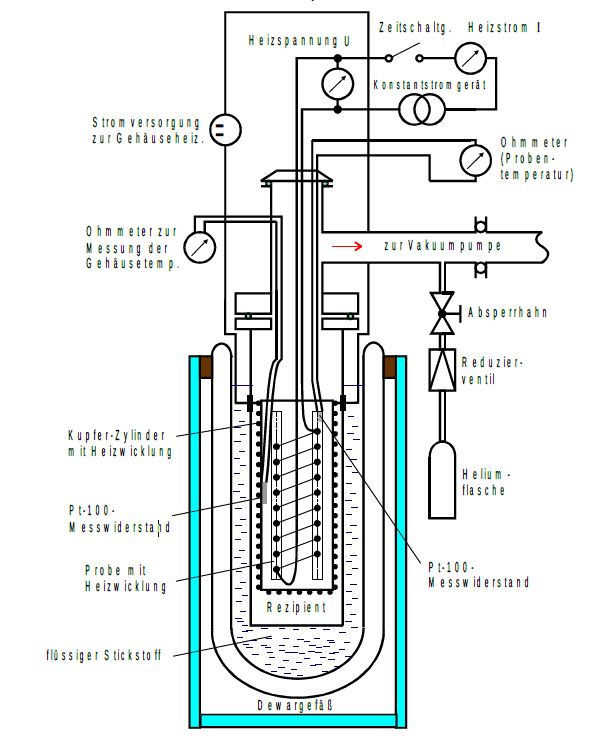
\includegraphics{build/Aufbau.jpg}
  \caption{Schematische Darstellung des Versuchsaufbau.\cite{Anleitung}}
  \label{fig:aufbau}
\end{figure}


\section{Durchführung}

Zu Beginn des Versuches wird etwaige Luft, die sich in Rezipienten befinden könnte, abgepumpt. Danach wird der Rezipient mit Helium befüllt. Damit wird sichergestellt das sich kein in der Luft enthaltendes Wasser in Rezipienten befindet und der Wärmeaustausch mit den Wärmebad möglichst gleichmäßig stattfinden kann. Das Dewar-Gefäß wird dann mit flüssigen Stickstoff befüllt. Nachdem die Probe auf ungefähr \SI{80}{\K} abgekühlt ist wird der Rezipient wieder evakuiert um den Wärmeaustausch der Probe mit seiner Umgebung möglichst gering zu halten.
Zum eigentlichen Messvorgang wird die Probe durch die sie umgebende Heißwickel erhitzt. Die Temperatur wird in gleichmäßigen Abständen von 1:30 Minuten gemessen. Zur Bestimmung der zugefügten Energie wird zudem die Spannung und Stromstärke, die an der Heizwicklung anliegt aufgenommen. Um einen Wärmeaustausch mit dem Rezipienten durch Wärmestrahlung zu vermeiden, wird dieser durch eine separate Heizwicklung gleichmäßig mit der Probe erhitzt. 
